%\large\zihao{-4}
%-----------------------------------------
\begin{center}
	{\heiti\bf\LARGE\zihao{3}{\biaoti\\}}
%	{\bf\LARGE\zihao{3}{\enbiaoti\\}}
%	{\enbiaoti}
	
	\vspace{0.3cm}
	{\heiti\bf\LARGE\zihao{-4}\minzi}
	
	{\zihao{5}\university\school,\city}
	
	{\zihao{5}zhongshengyanzy@foxmail.com}
\end{center}

%------------------------------------

%\begin{center}
%\begin{minipage}[t]{7cm}
\noindent{\zihao{5}{\bf 摘要:}
	\fangsong
	% 请填入中文摘要:
	夜间图像去雾技术作为计算机视觉领域研究的热点,有着许多广泛的应用,如智能车辆、交通监控、智慧感知等。近年来深度学习技术在图像去雾领域的应用十分火热,但主要集中于白天图像去雾,夜间图像去雾的主要研究方法仍以传统方法居多。我们综合了近年来国内外的研究工作,对现有应用深度学习技术处理夜间图像去雾任务的方法进行了详细的介绍,并指出了每种方法的优点和局限性,同时一步步地说明了深度学习技术在夜间图像去雾的潜力以及阻碍其发展的原因。最后展望了未来夜间图像去雾技术的研究方向,同时阐述了图像去雾技术的具体应用,希望吸引更多的研究人员关注到夜间图像去雾这一探索较少但十分重要的研究课题。
}\vspace{0.1cm}
%\end{minipage}
%\end{center}
%\end{multicols}
%\begin{multicols}{2} 
\begin{multicols}{2} 
\section{引言}\label{chpt:1}%===============================================

由于空气质量的下降和大气污染的加剧,近年来雾霾天气十分频发,空气中微粒对大气光的吸收与散射极易造成视野模糊和低能见度,给交通安全带来了极大的困扰,极大地影响了人们的出行与健康。此外,雾霾天气也对交通摄像头采集、信息识别、自动驾驶等造成了极大的干扰,设备采集图像的对比度与色彩大幅下降,图像质量严重退化,从而带来了图像模糊难以辨别、信息细节大幅丢失等问题。

图像去雾技术的发展有效地缓解了上述问题,通过设备算法植入的方式,在图像显示之前进行图像复原,能够有效地提高雾霾天气下图像的能见度和清晰度。但在夜间雾天环境下,由于光照不均,大气中悬浮的微粒对光的吸收和散射更为严重,直接造成图像细节丢失、颜色失真等现象,同时人工光源产生的辉光效应进一步带来了视线的干扰,容易产生光晕伪影等现象,这给图像去雾技术带来了极大的挑战,如何复原夜间雾霾环境下的图像目前仍然是一个十分棘手的问题。

近年来对图像去雾问题的研究十分火热,尤其是深度学习技术的应用,其优秀的性能和灵活的迁移能力有力推动了图像去雾技术的进步,但主要集中于白天图像去雾的应用。针对夜间图像去雾问题,近年来国内外众多研究人员仍主要集中于传统方法实现,深度学习技术的应用尝试还十分有限。而且由于夜间雾天图像干扰因素很众,目前尚没有统一的数学模型能够完整地表示夜间雾天的成像原理,也没有现有的方法可以对多个干扰因素同时获得表现良好的处理效果,可见该领域的研究潜力十分巨大。

区别于白天图像去雾,夜间雾天图像不仅仅只有雾霾的干扰,还增加了人造点光源、低照度、光照不均等多重干扰因素,在白天去雾中流行的大气散射模型\citeu{1}与暗通道先验等在夜间环境下均不再完全成立,于是研究者们开始希望通过改进传统的大气散射模型与先验,并通过融合、分层等多种手段实现图像去雾。Zhang et. al.\citeu{2},Li et. al.\citeu{3}均各自提出了改进的大气散射模型,考虑到了人造光源带来的辉光效应和颜色变化的影响,但由于未考虑到夜晚的不均匀照明,造成其出现颜色失真的问题;此外Pei et. al.\citeu{4}为了能够使用暗通道先验,首先对图像进行了颜色校正,力图使其拥有白天图像的颜色属性,但带来了低对比度、低亮度以及“蓝移”的色偏影响;Zhang et. al.\citeu{5}提出了一种统计先验,最大反射率先验(MRP)的方法,有效解决了存在变色和非均匀照明的情况下夜间图像的雾霾去除问题,但MRP是在每个像素的固定大小的邻域内使用,不能适应不同的局部统计,对于大面积的单色区域无法进行很好的处理;此外Liu et. al.\citeu{6}, Wang et. al.\citeu{7}, Wang et. al.\citeu{8}等采用分层、融合等方法,对辉光效应进行了显著地抑制与处理,但依然会有颜色失真与局部细节丢失的问题。

上述利用传统方法进行夜间图像去雾尽管已经取得了不错的效果,但是传统方法很难考虑到所有图像退化因素,而且易受到不同环境的影响。深度学习技术的引入为夜间图像去雾领域带来了新的活力,尽管至今研究文献较少,但现有的研究已证明了深度学习技术在夜间图像去雾的潜力巨大。主要阻碍深度学习技术在夜间图像去雾发展的因素是大规模数据集的缺乏,但Zhang et.al.\citeu{9}提出了一种称为$3R$的新型合成方法,能够从白天的清晰图像中模拟夜间的朦胧图像,它首先重建场景的几何形状,然后模拟光线和物体的反射率,最后渲染出朦胧效果,这为深度学习技术在夜间图像去雾领域的发展带来了巨大的帮助。同时计算机视觉上游任务网络框架的蓬勃发展更替如Transformer、ConvNet等也进一步地为下游任务带来启发与思考。

利用深度学习方法进行图像去雾主要分为两大类:1)通过深度学习方法估计物理模型中的未知参数进行图像去雾;2)从有雾图像到无雾图像端到端的去雾。本文主要对两种方法中的现有研究进行归纳和总结,详细阐述了现有方法的优势与不足,并对未来的研究方向进行了展望,最后介绍了图像去雾技术的具体应用与潜在挑战。


%\end{multicols}
%
%\begin{figure}[H]
%	\centering
%	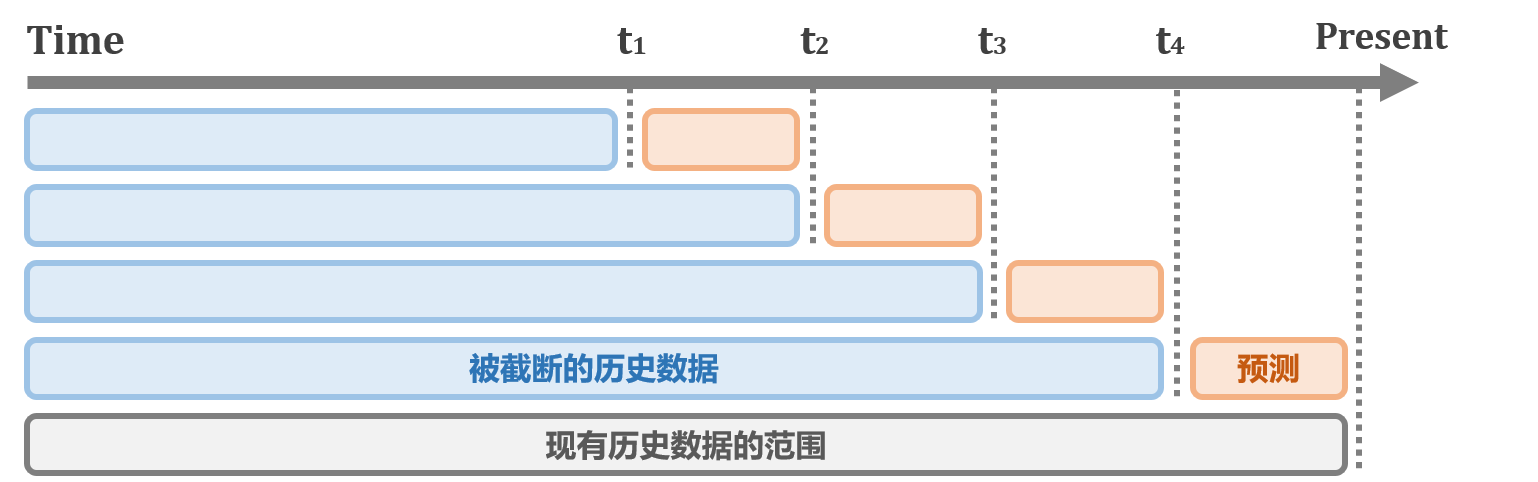
\includegraphics[width=14cm]{pics/bt1.png}\\
%	\caption{时间序列扩展窗口回测的概念示意图}\label{fig:backtest1}
%\end{figure}
%
%\begin{multicols}{2} 

%
%\begin{table}[H]
%	%\scriptsize
%	\footnotesize
%	\renewcommand{\arraystretch}{1.0}
%	\centering
%	\caption{\centering 模型的前移验证的预测评价指标统计对比}\label{tb:8}
%	\begin{tabular}{cccc}
%		\toprule[1.5pt]
%		&ARIMA&指数平滑&Prophet\\
%		\midrule[1pt]
%		 RMSE的中位数& 0.5440 &0.4785&\textbf{0.4055}\\
%		 RMSE的平均数& 0.5169&0.4529& \textbf{0.4126} \\
%		 MAE的中位数&0.4530 & 0.3435&\textbf{0.3045}\\
%		 MAE的平均值&0.4411 &\textbf{0.4115}&0.4116\\
%		 MAPE的中位数&108.84&92.38&\textbf{73.21}\\
%		 MAPE的平均值&134.32&119.56&\textbf{85.55}\\
%		\bottomrule[1.5pt]
%	\end{tabular}
%\end{table}
\section{相关工作}
\subsection{大气散射模型(ASM)}

Nayar S K et. al\cite{1} 最早提出了雾天成像的数学模型,该模型认为在强散射介质下,引起探测系统成像结果降质的主要原因有两种:一是目标反射光受大气中悬浮粒子的吸收和散射作用,造成目标反射光能量的衰减,这导致探测系统的成像结果亮度降低,对比度下降;二是太阳光等环境光受大气中散射介质的散射作用形成背景光,通常这部分背景光强度大于目标光,因而造成探测系统的成像结果模糊不清。具体成像过程如下图所示:
\begin{figure}[H]
	\centering
	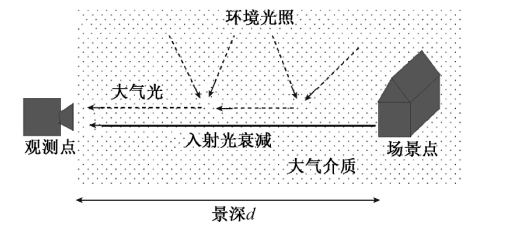
\includegraphics[width=0.9\linewidth]{pics/screenshot001}
	\caption{大气散射模型示意图}
	\label{fig:screenshot009}
\end{figure}
数学模型表达如下:
\begin{equation}
	I(x)=J(x)t(x)+A(1-t(x))
\end{equation}
其中$I(x)$表示有雾图像,$J(x)$表示无雾清晰图像,$A$表示大气光,$t(x)$表示光线的透射率,即光线在雾霾微粒中的穿透能力,取值在0$\sim$1之间,具体表达式为:
\begin{equation}
	t(x)=e^{-\beta d(x)}
\end{equation}
其中$\beta$和$d(x)$表示大气散射参数和场景深度,这也意味着$t(x)$可以通过场景深度图$d(x)$得到,这有助于合成数据集。如果我们得到$t(x)$和$A$的估计值,则清晰无雾图像可表示为:
\begin{equation}
	J(x) = \frac{I(x)-A(1-t(x))}{t(x)}
\end{equation}

所有白天的图像去雾方法,例如暗通道先验(DCP)\cite{10}和夜间图像去雾初期的一些研究工作\cite{3}\cite{11}都是按照这个模型设计的。这个模型的确准确地表现了白天的雾霾图像,因为它认为图像的大气光是全局均匀的,这完全符合白天图像的照明特性。但它不能同样完美地表现夜间图像,因为夜间图像通常具有空间变化的照度特征,同时这个模型也不包含任何用于表示夜间图像发光特性的参数项。所以之所以按照这个模型设计的方法常常产生含有光晕伪影的彩色扭曲输出图像,因为它们不能有效地处理空间变化的照明特征以及辉光效应等发光特征。为了克服这些缺点,\cite{2}\cite{3}\cite{12}中的作者提出了几个夜间雾霾图像的成像模型,以准确表示夜间雾霾图像的特征。

\subsection{夜间图像去雾任务数据集}
针对深度学习技术在夜间图像去雾任务上的应用,Zhang等人\cite{5}通过添加单一的黄色恒定中心光源,根据Middlebury数据集\cite{13}合成了夜间的雾霾图像;此外,Zhang et.al.\cite{9}对真实世界的光照颜色进行了实证研究,获得其颜色分布,基于此提出了一种新的合成方法$3R$,进一步考虑到了场景的深度和几何性质,通过同时渲染空间变化的偏色和雾霾来生成真实的夜间阴霾图像,生成的数据集参数见表\ref{tb:8}。
\begin{table}[H]
	%\scriptsize
	\footnotesize
	\renewcommand{\arraystretch}{1.0}
	\centering
	\caption{\centering 数据集的统计数据}\label{tb:8}
	\begin{tabular}{cccc}
		\toprule[1.5pt]数据集
		&雾霾密度&数量&合成的\\
		\midrule[1pt]
		 NHC-L& 薄雾 &2750&$\checkmark$\\
		 NHC-M& 中等&2750& $\checkmark$ \\
		 NHC-D& 浓雾&2750& $\checkmark$ \\
		 NHM& 均有&350& $\checkmark$ \\
		 NHR& 均有&8970& $\checkmark$ \\
		 NHRW& 均有&150& $\times$ \\
		\bottomrule[1.5pt]
	\end{tabular}
\end{table}

\subsection{图像质量衡量标准}
在图像去雾领域最常用的客观评价指标有如下几种:
\begin{enumerate}
	\item[(1)] 峰值信噪比(Peak Signal To Noise
	Ratio, PSNR)\cite{15}
	
	PSNR常常用来衡量修复后的无雾图像的质量,PSNR越高,失真越小。其数学表示如下:
	\begin{equation}
		PSNR=10log_{10}(\frac{Max^2}{MSE})
	\end{equation}
	其中$Max$表示图像点颜色的最大数值,如果每个采样点用8位表示,则取255;$MSE$为真实图像和输出图像之间的均方误差,表达式为:
	\begin{equation}
		MSE=\frac{1}{M_1\times N_1}\sum_{i=1}^{M_1}\sum_{j=1}^{N_1}|GT(i,j)-J(i,j)|^2
	\end{equation}
	\item[(2)]结构相似性(Structure Similarity Index Measure, SSIM)\cite{14}
	
	SSIM主要考量图片的三个关键特征:亮度(Luminance), 对比度(Contrast), 结构(Structure)。这个定量参数主要衡量输出图像和相应的真实图像之间的结构相似性。与MSE和PSNR衡量绝对误差不同,SSIM是感知模型,即更符合人眼的直观感受。它的值在0$\sim$1之间。SSIM值越接近1则标志着图像之间的高相似度。在数学上,这个参数表示如下:
	\begin{equation}
		\footnotesize{
		SSIM(GT,J)=\frac{(2\mu_{GT}\mu{J}+C_1)(2\sigma_{GT,J}+C_2)}{(\mu_{GT}^2+\mu_J^2+C_1)(\sigma_{GT}^2+\sigma_J^2+C_2)}}
	\end{equation}
	\item[(3)] CIEDE2000\cite{16}
	
	这个参数衡量真实图像和输出图像之间的色差。因此,零是这个参数的理想结果,即表示完美的色彩修复。但在实际情况下,它的值往往大于零。
	
\end{enumerate}
\section{基于深度学习的夜间图像去雾方法}
利用深度学习方法进行夜间图像去雾主要分为两大类:
% TODO: \usepackage{graphicx} required
% TODO: \usepackage{graphicx} required
\begin{figure}[H]
	\centering
	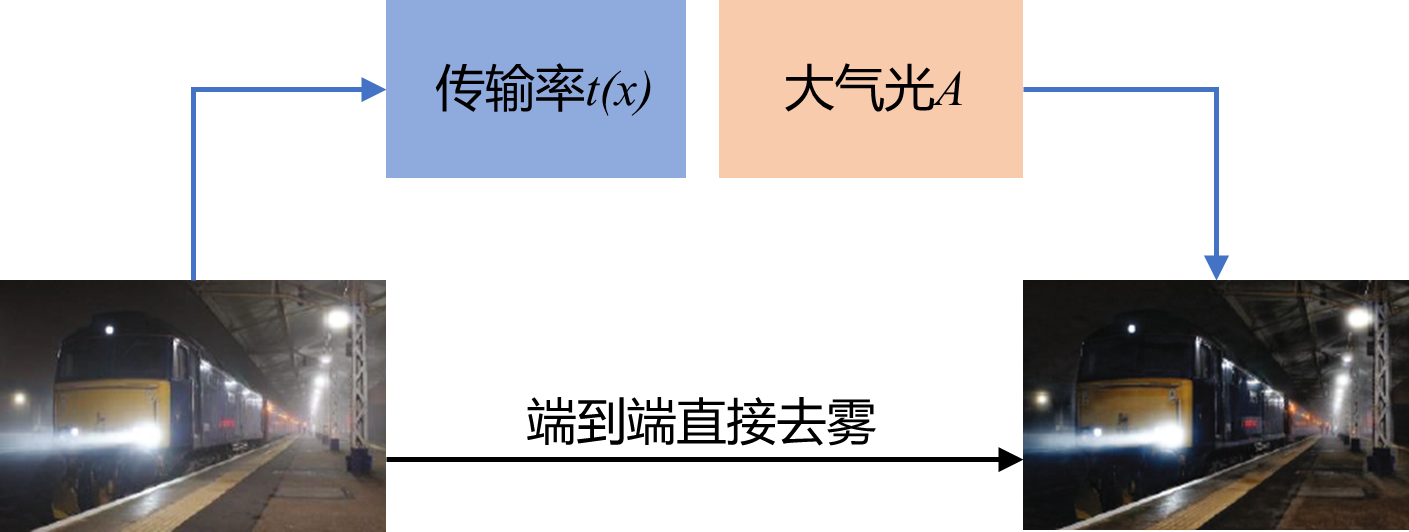
\includegraphics[width=1.0\linewidth]{pics/screenshot011}
	\caption{利用深度学习方法进行夜间图像去雾的工作流程}
	\label{fig:screenshot011}
\end{figure}

\begin{itemize}
	\item 通过深度学习方法估计夜间成像物理模型中的未知参数进行图像去雾
	
	该类方法将大气散射模型与神经网络相结合,通过估计物理模型中的未知参数如$t(x),A$等,再根据大气散射模型$I(x)=J(x)t(x)+A(1-t(x))$或其他改进模型得到最后的无雾清晰图像。
	\item 通过深度学习方法学习从有雾图像到无雾图像的映射关系,实现端到端的直接去雾
	
	该类方法无需依赖物理成像模型,跳过了参数估计的步骤,力图直接获取有雾图像和无雾图像之间的映射关系,从而直接输出清晰无雾图像,但需要成对的数据进行训练。
\end{itemize}

下面对这两类中的现有研究进行介绍论述。
\subsection{基于物理模型的去雾方法}
\noindent\textbf{用于夜间图像去雾的卷积自动编码器}

Feng. et al.\cite{17}在处理夜间有雾图像时,沿用了传统的大气散射模型,采用了传统方法与深度学习相结合的方案,将整个去雾任务划分为三个步骤:颜色校正、传输率估计、大气光照估计,最后再根据(3)进行图像复原。

作者首先使用了MRP\cite{5}对图像进行颜色校正的预处理。根据Retinux理论\cite{18}和\cite{5}中的分析,将大气散射模型(1)式重写为:
\begin{equation}
	I(x)\triangleq L(x)\eta(x)R(x)t(x)+L(x)\eta(x)(1-t(x))
\end{equation}
其中$L(x)$表示环境光照强度,$R(x)$表示场景反射率,$\eta(x)$表示环境光照的颜色。

又由于\cite{5}中假设在同一图像分割块中环境照度、光照强度、颜色图谱以及传输率$t(x)$的值是恒定一致的。所以对(7)式两边同时取最大值,可得:
\begin{equation}
	M_{\Omega_i}^c=\mathop{\max}_{j\in \Omega_i} I_j^c = \mathop{\max}_{j\in \Omega_i} R_j^c(L_{\Omega_i} \eta_{\Omega_i^c}t_{\Omega_i})+L_{\Omega_i}\eta_{\Omega_i^c}(1-t_{\Omega_i})
\end{equation}
其中$M_{\Omega_i}^c$即表示在图像分割块$\Omega_i$通道$c$中的最大像素值,$c\in (r,g,b)$。又因为在\cite{5}中有如下定义
\begin{equation}
	\mathop{\max}_{x\in \Omega_i} R(x)^c\approx 1
\end{equation}
所以可得到以下表达式:
\begin{equation}
	M_{\Omega_i}^c=L_{\Omega_i} \eta_{\Omega_f^c}t_{\Omega_i}+L_{\Omega_i}\eta_{\Omega_i^c}(1-t_{\Omega_i})=L_{\Omega_i} \eta_{\Omega_i^c}
\end{equation}
通过式(10),便可估计环境光照的颜色图谱:
\begin{equation}
	 \eta_{\Omega_i^c} = \frac{M_{\Omega_i}^c}{L_{\Omega_i}}
\end{equation}
进而最终通过下式消除了环境光照颜色的影响。
\begin{equation}
	\hat{I_j^c}\triangleq\frac{I_j^c}{\eta_{\Omega_i^c}}
\end{equation}
其中$\hat{I_j^c}$即表示消除了颜色影响的雾霾图像。

在进行颜色校正后,考虑到传统物理先验在不同的场景往往会出现高估或低估传输率的问题,Feng. et 
\end{multicols}
\begin{figure}[H]
\centering
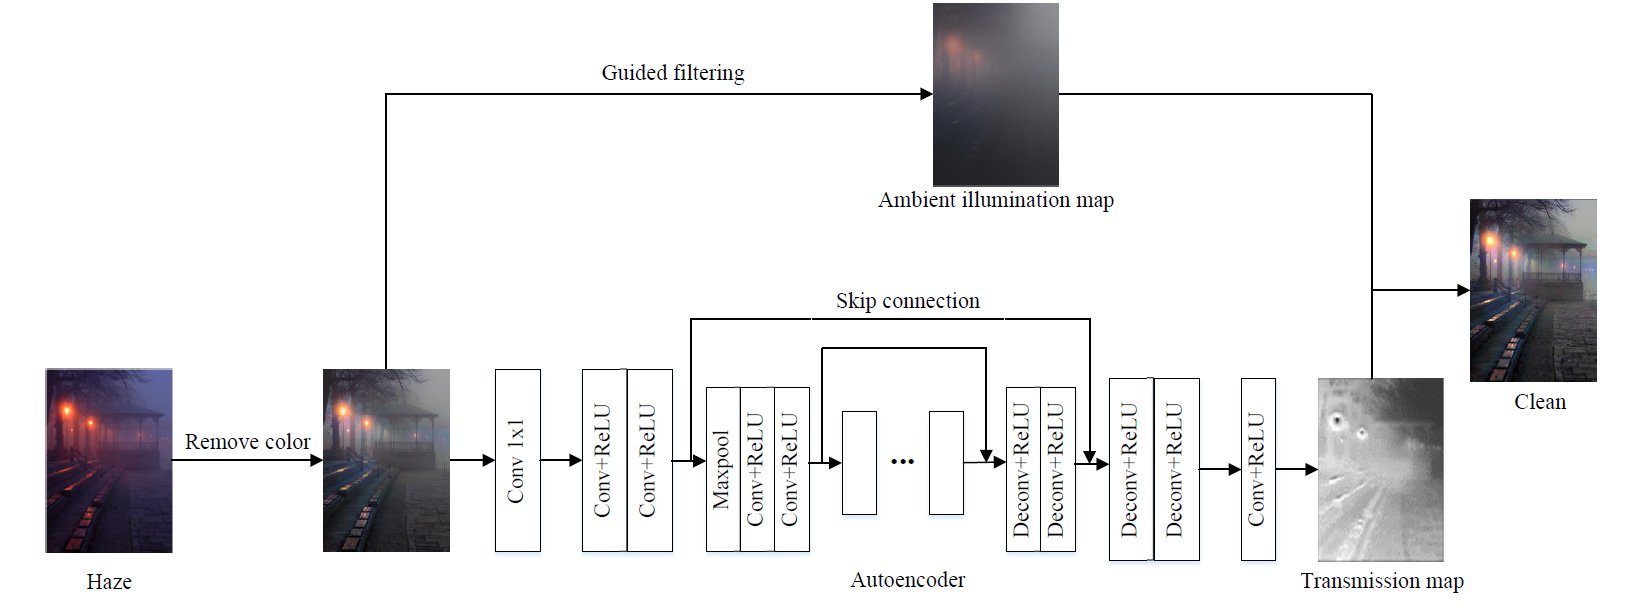
\includegraphics[width=1.0\linewidth]{pics/screenshot002}
\caption{Feng.等人提出的夜间图像去雾方法}
\label{fig:screenshot002}
\end{figure}
\begin{multicols}{2}
\noindent al.\cite{17}利用了一种简单的自编码器网络,并引入了残差连接,更好地降低了图像模糊的程度,同时获得更多的纹理细节特征。小尺寸卷积核的引入可以保留更多的局部信息,减少了过程中的信息衰减。具体的网络结构见图\ref{fig:screenshot002},编码器和解码器的具体信息见表\ref{tb:9},\ref{tb:10}。损失函数为
\begin{equation}
	Loss_T=MSE(T,T_{gt})
\end{equation}
其中$T$代表自编码器网络输出的传输率图像,$T_{gt}$代表真实图像的传输率图。


\begin{table}[H]
	\scriptsize
	%\footnotesize
	\renewcommand{\arraystretch}{1.0}
	\centering
	\caption{\centering 编码器的具体信息}\label{tb:9}
	\begin{tabular}{ccccc}
		\toprule[1.5pt]	Activation Size & Kernel Size & Stride & Padding & Max-Pooling \\
		\midrule[1pt]
		3$\times$256 $\times$256   & 64$\times$3$\times$3  & 1      & 1       & ——          \\
		64$\times$256 $\times$256      & 64$\times$3$\times$3   & 1      & 1       & 2           \\
		64$\times$128$\times$128      & 128$\times$3$\times$3 & 1      & 1       &  ——         \\
		128$\times$128$\times$128     & 128$\times$3$\times$3 & 1      & 1       & 2           \\
		128$\times$64$\times$64       & 256$\times$3$\times$3 & 1      & 1       & ——           \\
		256$\times$64$\times$64   & 256$\times$3$\times$3 & 1      & 1       & 2           \\
		256$\times$32$\times$32   & 512$\times$3$\times$3 & 1      & 1       &  ——           \\
		512$\times$32$\times$32   & 512$\times$3$\times$3 & 1      & 1       & 2           \\
		512$\times$16$\times$16    & 512$\times$3$\times$3  & 1      & 1       &  ——           \\
		512$\times$16$\times$16       & 512$\times$3$\times$3 & 1      & 1       &  ——      \\    
		\bottomrule[1.5pt]
	\end{tabular}
\end{table}
\begin{table}[H]
	\scriptsize
	%\footnotesize
	\renewcommand{\arraystretch}{1.0}
	\centering
	\caption{\centering 解码器的具体信息}\label{tb:10}
	\begin{tabular}{ccccc}
		\toprule[1.5pt]	Activation Size & Up-Sampled & Kernel Size & Stride & Padding \\
		\midrule[1pt]
		512$\times$16$\times$16       & 2          & 256$\times$3$\times$3 & 1      & 1       \\
		256$\times$32$\times$32   & ——           & 256$\times$3$\times$3 & 1      & 1       \\
		256$\times$32$\times$32   & 2          & 128$\times$3$\times$3 & 1      & 1       \\
		128$\times$64$\times$64    &    ——        & 128$\times$3$\times$3 & 1      & 1       \\
		128$\times$64$\times$64       & 2          & 64$\times$3$\times$3  & 1      & 1       \\
		64$\times$128$\times$128      &  ——          & 64$\times$3$\times$3  & 1      & 1       \\
		64$\times$128$\times$128      & 2          & 64$\times$3$\times$3   & 1      & 1       \\
		64$\times$256$\times$256      &  ——          & 64$\times$3$\times$3   & 1      & 1       \\
		64$\times$256$\times$256      &  ——          & 1$\times$1$\times$ 1   & 1      & 0      \\ 
		\bottomrule[1.5pt]
	\end{tabular}
\end{table}
Feng. et al.使用自编码器网络估计传输率的方式,有效解决了传统先验知识在夜间不完全成立的问题,提高了模型的精度与鲁棒性。得到传输率图$t(x)$后,作者再通过一种低通导向滤波的方法对大气光照$A$进行估计,最后根据式(3)即得到最终的无雾图像。具体去雾效果如下所示:
% TODO: \usepackage{graphicx} required
\begin{figure}[H]
	\centering
	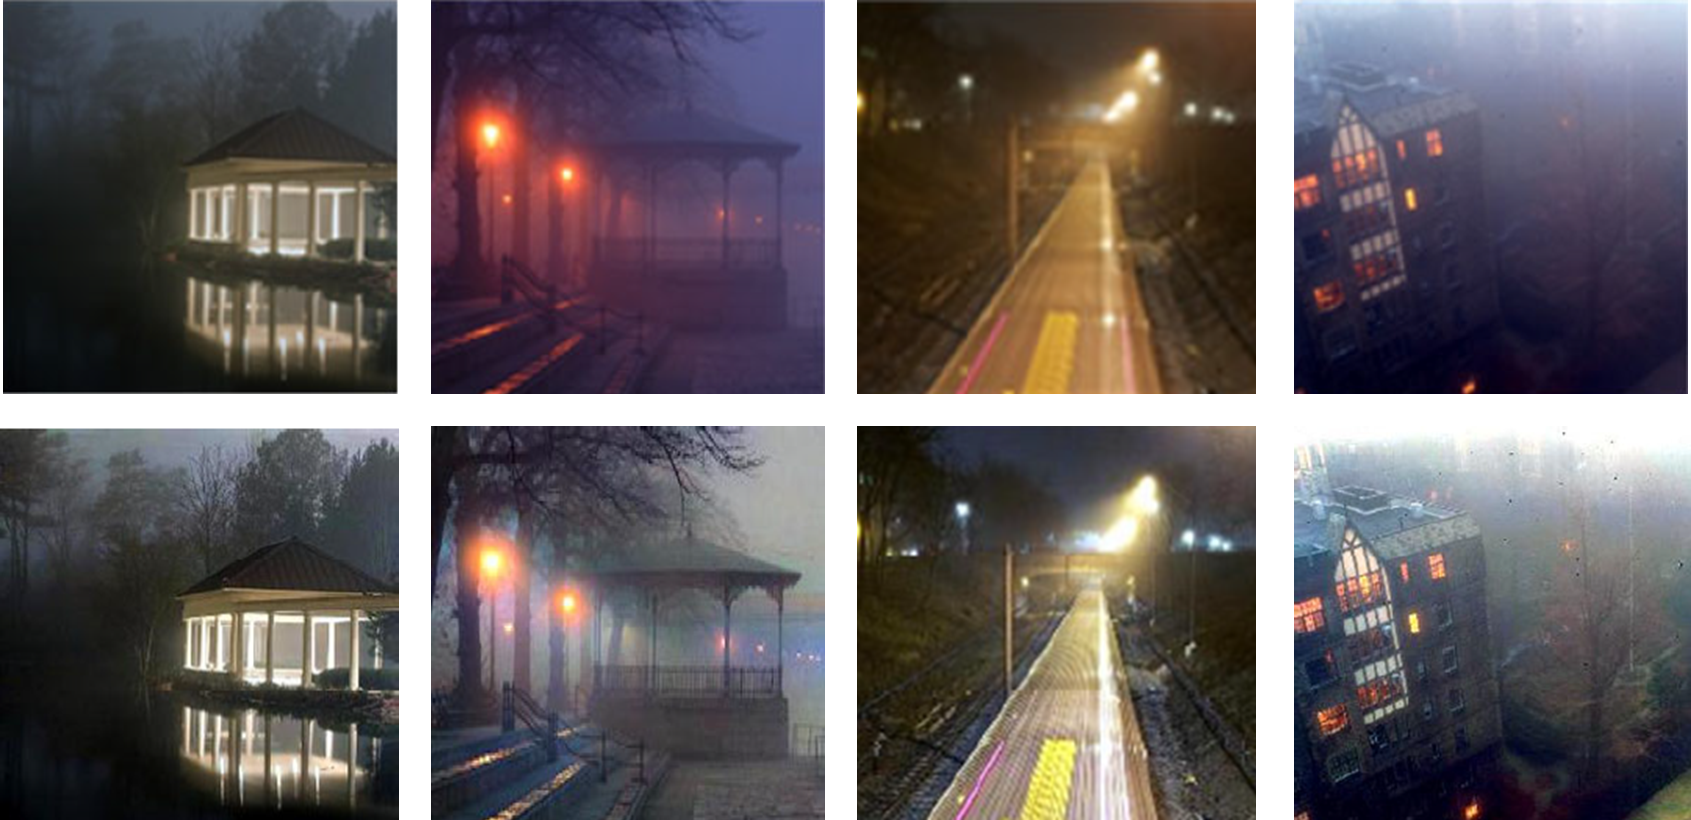
\includegraphics[width=1.0\linewidth]{pics/screenshot012}
	\caption{在真实夜间雾天数据集上的去雾效果}
	\label{fig:screenshot012}
\end{figure}

结果表明,自编码器网络的应用与传统方法的结合显著地实现了去雾效果,很好地保留了光源附近的细节特征,同时提高了图像的能见度;但仍存在颜色轻度失真、局部纹理细节损失的问题,这主要是因为在颜色校正的过程中可能出现了过度校正的问题,此外由于物理模型中并未考虑到辉光效应,所以光源附近的参数估计存在一定的误差。


\noindent\textbf{用于夜间图像去雾与去辉光的多路膨胀卷积网络}

Kuanar et al. \cite{20} 设计了如图\ref{fig:screenshot004}所示的网络用来进行夜间雾天图像的辉光效应去除。他们考虑到了夜间图像中的辉光效应等发光特征,故提出了改进的大气散射模型,在传统的大气散射模型上增添了辉光参
\end{multicols}
% TODO: \usepackage{graphicx} required
\begin{figure}[H]
\centering
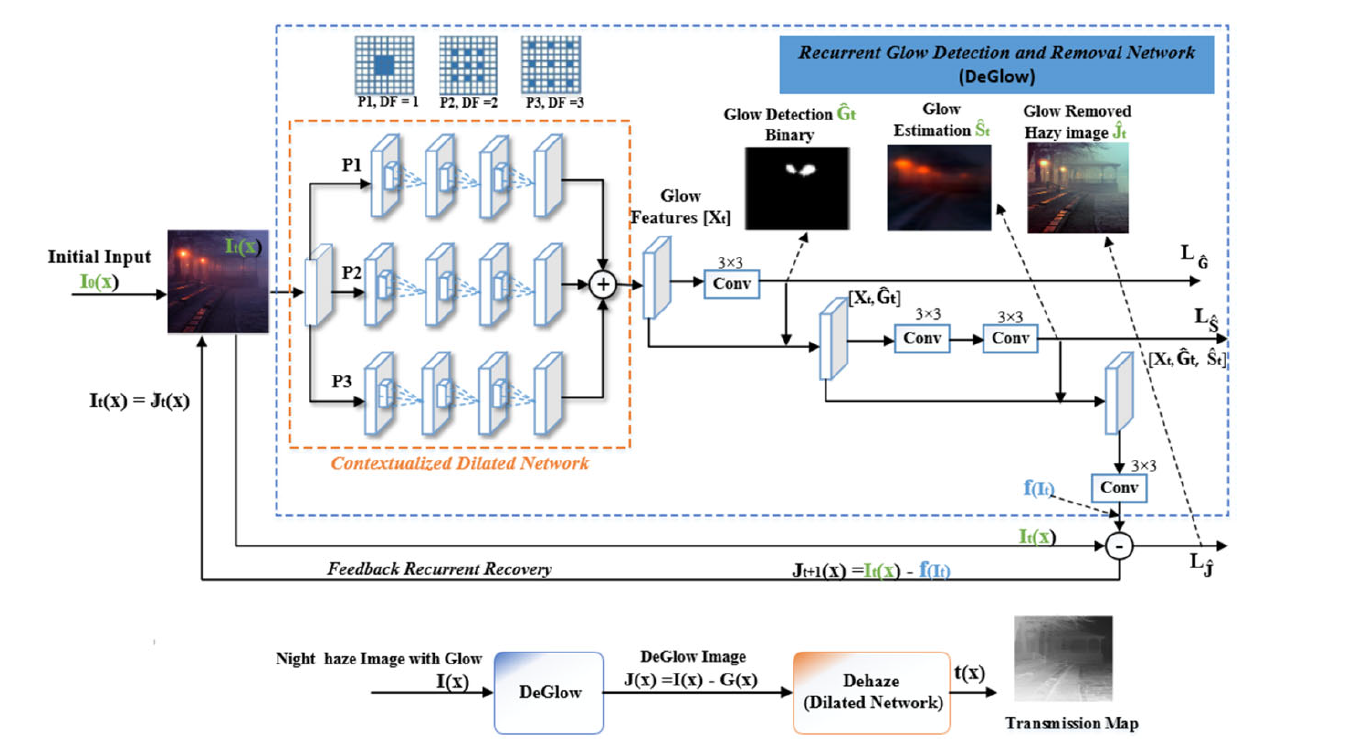
\includegraphics[width=0.9\linewidth]{pics/screenshot004}
\caption{Kuanar 等人提出的DeGlow网络结构}
\label{fig:screenshot004}
\end{figure}
\begin{multicols}{2}
\noindent 数项:
\begin{equation}
	I(x)=J(x)t(x)+A(1-t(x))+\sum_{k=1}^{n}\hat{S_k(x)}*\hat{G}
\end{equation}
其中前两项即为传统的大气散射模型,第三项则为辉光项,用来表示图像中出现的辉光效应。$\hat{S_k(x)}$代表一个辉光源的形状和照明方向,下标$k$代表重叠的辉光数,范围从1到$n$,其中$n$是大气中辉光源的数量。变量$\hat{G}$表示图像区域上的可见辉光点,采取二进制掩码,其中$\hat{G}=1$则表示辉光区域,反之为非辉光区域。
这样的设计一方面有利于提供额外的信息来检测发光区域,另一方面又允许网络分别作用于辉光区域和非辉光区域,而不会影响雾霾图像的背景纹理细节。

整个网络结构分为DeGlow和DeHaze两重网络。DeGlow网络使用循环学习的多路径膨胀卷积网络提取辉光特征,三条路径P1,P2,P3均拥有三个3*3核卷积层,但是膨胀卷积因子(DF)不尽相同,分别为P1:DF=1,P1:DF=2,P1:DF=3,这样的设计可以获取更大的感受野,防止局部细节与分辨率的过分丢失,促进了更多纹理细节的保留与聚合。

\end{multicols}

% TODO: \usepackage{graphicx} required
\begin{figure}[H]
\centering
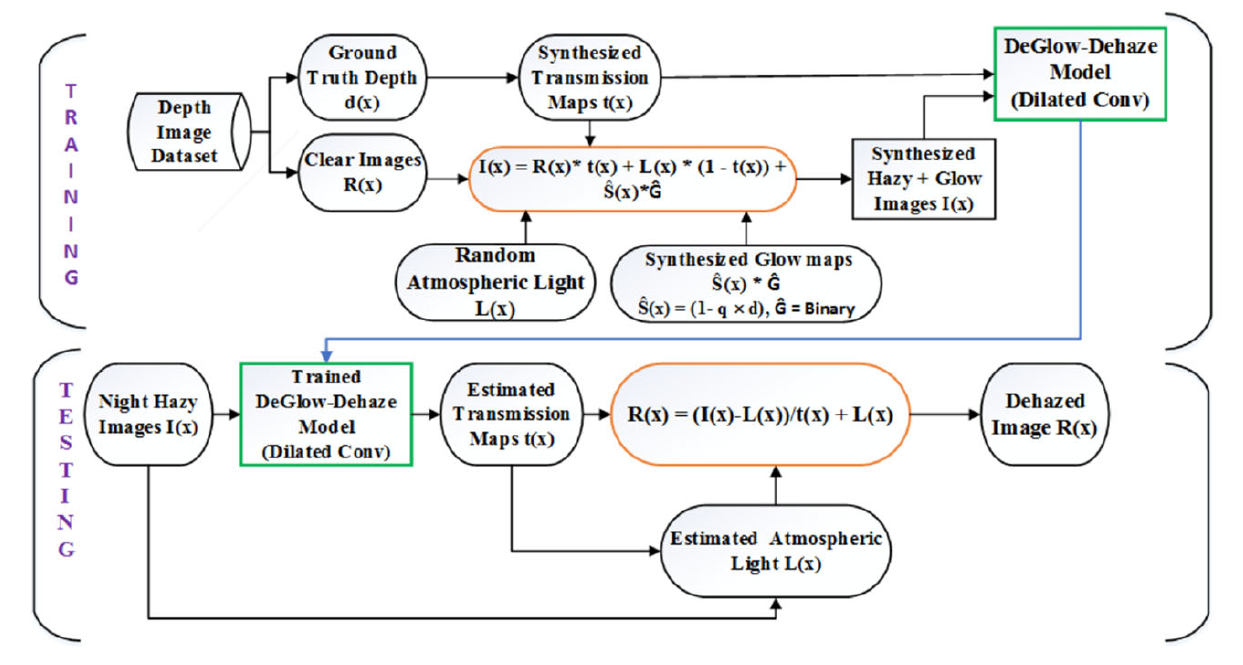
\includegraphics[width=0.75\linewidth]{pics/screenshot005}
\caption{DeGlow-DeHaze网络的工作流程}
\label{fig:screenshot005}
\end{figure}
\begin{multicols}{2}
在辉光效应去除后,作者利用一个与DeGlow网络相似的DeHaze网络进行去雾,区别仅在于该网络只有一次循环,对传输率图的估计方法与\cite{21}类似。而对大气光照的估计,作者沿用了白天去雾的思路,认为大气光照是全局均匀的,以上一步得到的估计透射率图中的0.1\%的最亮像素点强度的平均值作为大气光的估计值。最后再根据物理模型即可得到无雾图像。整个工作的流程如图\ref{fig:screenshot005}所示。

DeGlow-DeHaze网络对膨胀卷积网络的巧妙运用不仅消除了辉光效应的影响,同时使得局部纹理细节和图像分辨率得以很好地保持。同时网络同时可作用于辉光区域与非辉光区域,避免了背景信息的损失与退化。但由于夜间的环境光照受到人工光源的影响并非是完全均匀的,所以该模型对于大气光的估计存在一定的误差,从而会产生颜色失真,图像整体偏暗的影响。

\end{multicols}

% TODO: \usepackage{graphicx} required
\begin{figure}[H]
	\centering
	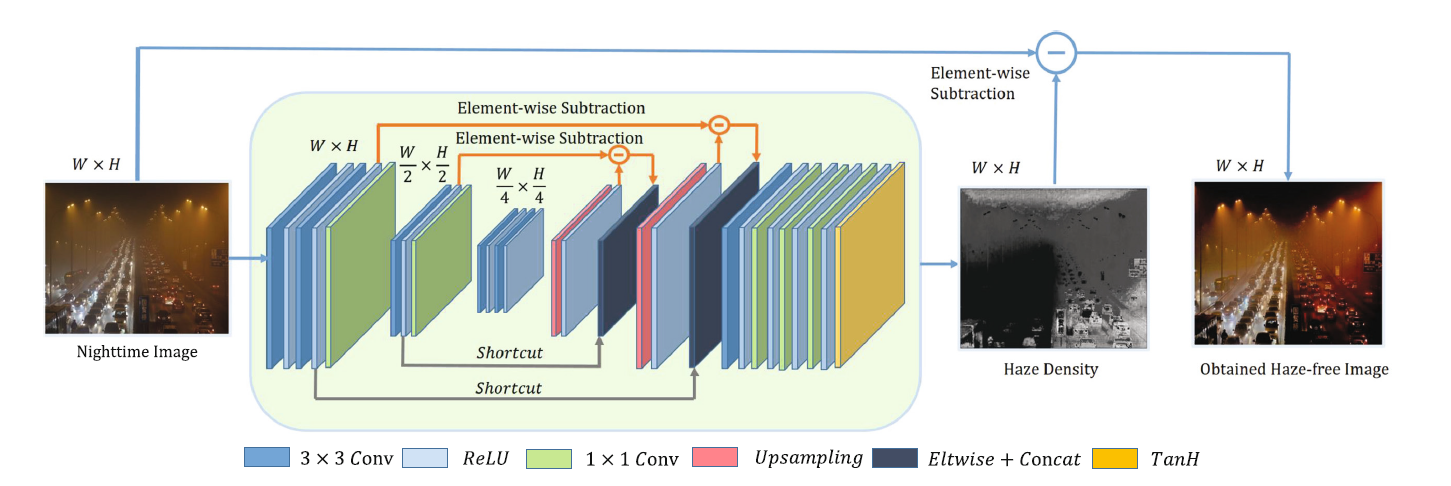
\includegraphics[width=1.0\linewidth]{pics/screenshot006}
	\caption{Liao 等人提出的HDP-Net去雾网络}
	\label{fig:screenshot006}
\end{figure}

\begin{multicols}{2}
\subsection{端到端的直接去雾方法}
\noindent\textbf{用于夜间去雾的雾霾密度预测网络}

Liao et al.\cite{22}提出了一种雾霾密度预测网络,不同于\cite{20}对中间参数进行预测的方式,该网络力图直接通过端到端的方式完成图像去雾。

作者首先设计了一种雾霾密度预测(Haze Density Prediction, HDP)函数:
\begin{equation}
	I_h=P(I(x))
\end{equation}
其中$I_h$表示雾密度,$P(·)$表示预测函数,基于此作者将大气散射模型进行改写:
\begin{equation}
	I(x)=J_s(x)+J_t(x)+I_h(x)
\end{equation}
其中$J_s(x)$和$J_t(x)$分别表示无雾图像的结构层和纹理层,所以只需要得到雾密度,便可直接获得无雾图像。作者通过证明得到雾密度的范围为[-1,1],并论证了去雾方法的合理性。

然后作者设计了如图\ref{fig:screenshot006}所示的网络结构用来预测图像的雾密度图,整体网络结构与全连接神经网络(Fully Connected Network, FCN)类似,也有效地应对了不同环境下雾霾的分布与密度差异。网络结构中同样引入了残差连接,以保留更多的图像颜色与细节纹理特征。具体的网络层信息见表,中间层均采用了Relu激活函数,借其稀疏特性减少空间复杂度,而最后输出层采用了Tanh激活函数,也刚好满足了雾密度的取值范围为[-1,1]。网络的损失函数如下:
\begin{equation}
	Loss=\sum \Vert J-(I-I_{conv}) \Vert_2
\end{equation}
具体效果如下所示:
% TODO: \usepackage{graphicx} required
\begin{figure}[H]
	\centering
	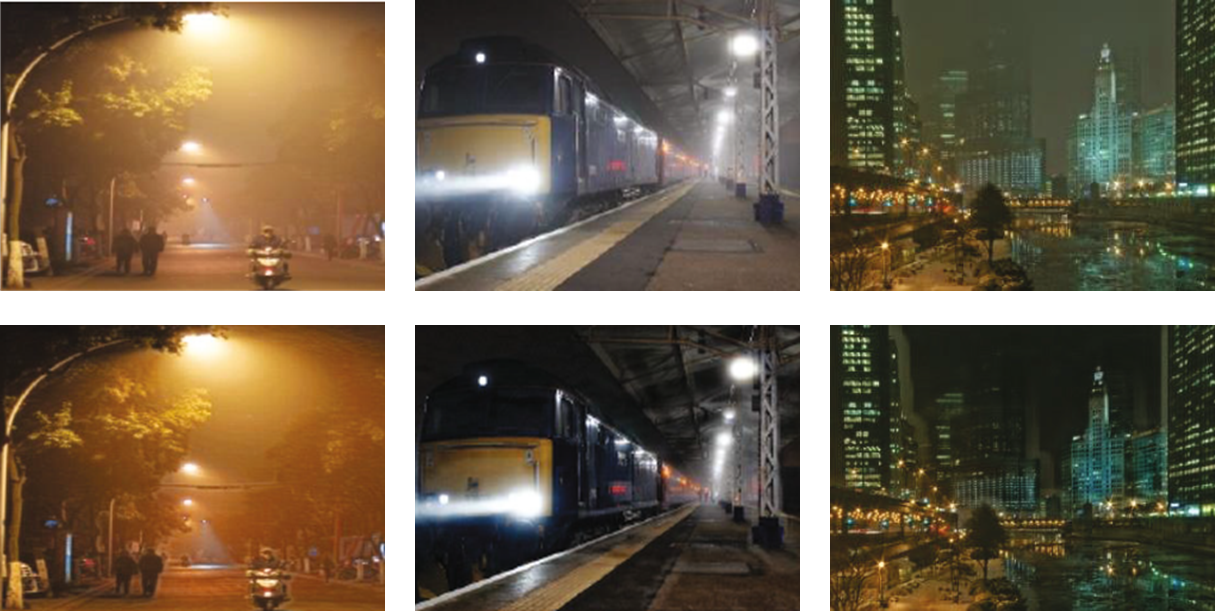
\includegraphics[width=1.0\linewidth]{pics/screenshot013}
	\caption{真实夜间雾天图像去雾效果}
	\label{fig:screenshot013}
\end{figure}


Liao et al.\cite{22}的方法可以实现直接端到端的去
\end{multicols}
\begin{figure}[H]
\centering
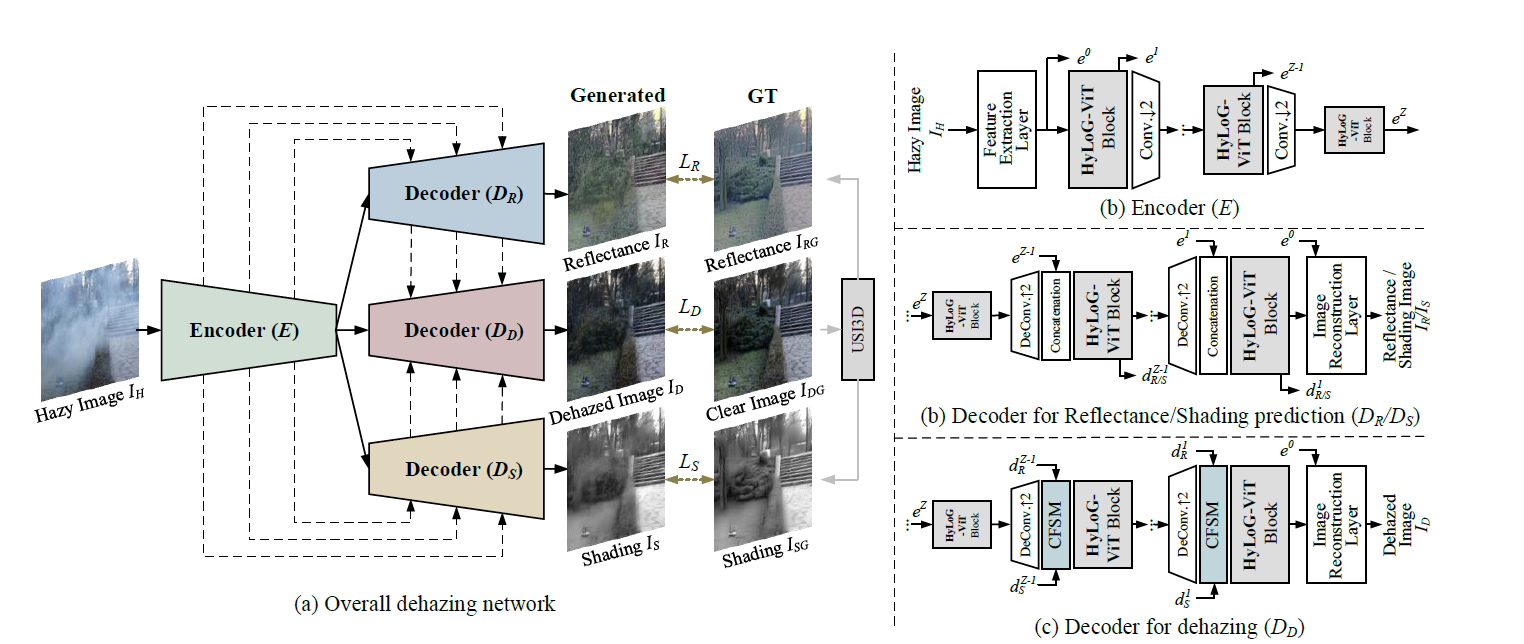
\includegraphics[width=1.0\linewidth]{pics/screenshot007}
\caption{Zhao 等人提出的去雾网络框架}
\label{fig:screenshot007}
\end{figure}

\begin{multicols}{2}

\noindent 雾,有效降低了计算负担;同时类似全连接网络的设计提高了算法的鲁棒性,使得对不同分布、不同密度雾霾的图像均有不错的表现;但在有变化光源和辉光效应的图像上很难准确地估计雾密度图,从而会容易造成扭曲和局部信息的丢失的现象。

\noindent\textbf{基于Vision Transformer的互补特征增强网络}

 Zhao et. al.\cite{23}设计了如图\ref{fig:screenshot007}所示的去雾网络,可同时运用于白天去雾和夜间去雾任务。
 
 不同于传统CNN隐式地学习特征,该网络直接有目的的学习特定的任务,作者通过严谨的分析论证选择了本征图像分解作为互补任务,其中反射图和光照度预测两个子任务可分别用来提取颜色和纹理特征,极大程度上保留了图像的细节信息与颜色特征。
 
 此外,为了有效地聚合这些互补特征,作者提出了一个互补特征选择模块(Complementary Features Selection Module, CFSM)用来选择对去雾工作更有用的特征,具体设计如下图所示,CFSM利用了全局平均和最大池化的方式来自适应地增强适当的互补特征通道,同时削弱不相关的特征通道,大大地提高了特征聚合的有效性。
 
 作者还提出了一种Vision Transformer的新变种,Hybrid Local-Global Vision Transformer(HyLoG-ViT),它能够以比普通ViT模型更低的计算成本来获取局部和全局的依赖关系,从而加速了模型的训练速度,同时使得复原图像更加地自然,局部细节特征复原更加清晰。其具体框架如下图所示:

 \begin{figure}[H]
 	\centering
 	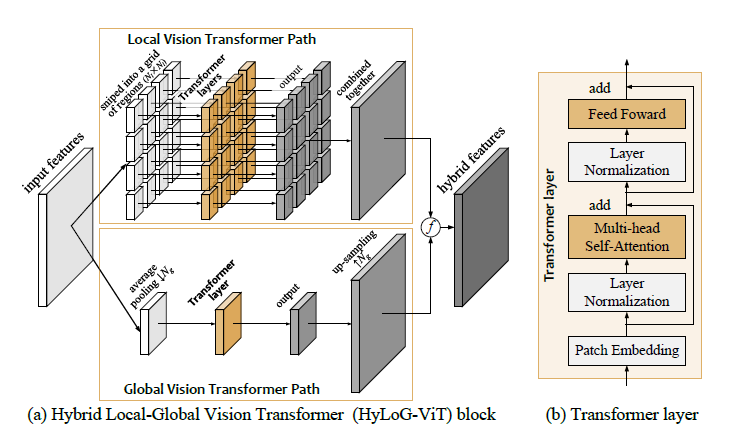
\includegraphics[width=1.0\linewidth]{pics/screenshot008}
 	\caption{HyLoG-ViT的架构示意图}
 	\label{fig:screenshot008}
 \end{figure}
 

\section{未来的挑战与机遇}
\begin{itemize}
	\item 从以上综述结果看,目前仍然没有方法可以在真实夜间雾天图像上表现效果良好,如何提高算法的泛化能力依旧是亟待解决的问题。
	\item 从深度学习技术在夜间图像去雾领域目前的表现来看,其发展的潜力仍然巨大,但大规模数据集与真实图像数据集的缺乏依旧是该领域发展的极大阻碍。
	\item 现有的模型难以同时考虑到所有图像退化因素,如何设计出集图像增强、图像去雾、图像去辉光等一体化,同时又能够做到轻量化的网络也是值得思考的问题。
	\item 深度学习技术发展迅速,新的模型层出不穷,如何将上游任务中的先进网络迁移到下游任务,同时提高模型的训练速度,也是未来研究的重点任务。
	\item 现有的图像去雾技术很难做到可以同时应对白天去雾与夜间去雾任务,如何设计出能够对环境自适应辨别的通用性网络依旧是一个很大的挑战。
\end{itemize}

\section{图像去雾技术的具体应用场景}
\begin{itemize}
	\item 辅助驾驶系统
	
	近年来,辅助驾驶行业蓬勃发展,但恶劣天气状况下驾驶员的行车视觉干扰问题一直没有比较好的解决方案,随着图像去雾技术的发展,通过在车前方安装相应的显示设备,在恶劣天气时,能够实时显示车前方路况的去雾图像,从而辅助驾驶员获得更清晰的视野,降低了行车的安全风险。
	
	\item 交通监控系统
	
	在夜间、雾霾天气等能见度较低的场景下,往往监控摄像头拍摄的景象辨识度极低,这不利于交通监管与社会治安的工作开展。向摄像头中搭载计算芯片,植入图像去雾与图像增强算法,便可提高拍摄画面的能见度,从而帮助交通监管获得更清晰的视野,也便于提高车牌识别等上游任务的精度。
	
	\item 无人车与无人驾驶
	
	对于现有的无人驾驶技术,或流行的无人物流小车等,恶劣天气均是智能感知的一大障碍,不利的能见度与辨识度容易造成系统的判断失误与决策混乱,这无疑是风险极大的。随着图像去雾、去雨等算法的发展,未来智能感知系统会更加完善,在恶劣天气下的视觉捕捉也能够得到实时的清晰化,这有助于提高无人系统的精度和可信度。
	
\end{itemize}
\section{总结}
本文我们主要针对深度学习技术在夜间图像去雾领域的应用作了详细的介绍与论述,分别从基于物理模型的参数估计方法和端到端的直接去雾方法两类实现方式分析了现有技术的优势与不足,同时指出了夜间图像去雾相比白天图像去雾的区别与难点,以及现阶段仍然存在的挑战和对未来的展望,并在最后简单阐述了图像去雾技术的实际应用场景。

\end{multicols}




















